% HEXA GRAPH

\documentclass[border=5, varwidth]{standalone}

\usepackage{tikz}

\begin{document}

    % Round 1
    Round 1:
    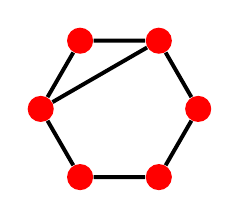
\begin{tikzpicture}[
            scale = 1,
            every node/.style={transform shape, text depth=0pt, circle},
            line/.style={line width = .05cm},
            ]
        
        \node[fill=red] (1) at (0: 1cm) {};
        \node[fill=red] (2) at (60: 1cm) {};
        \node[fill=red] (3) at (120: 1cm) {};
        \node[fill=red] (4) at (180: 1cm) {};
        \node[fill=red] (5) at (240: 1cm) {};
        \node[fill=red] (6) at (300: 1cm) {};
        
        \draw[line] (1) -- (2) -- (3) -- (4) -- (5) -- (6) -- (1);
        \draw[line] (4) -- (2);
    \end{tikzpicture}
    \\[1cm]
    % Round 2
    Round 2:
    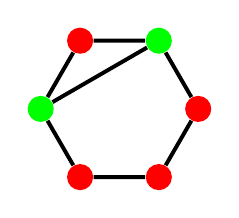
\begin{tikzpicture}[
            scale = 1,
            every node/.style={transform shape, text depth=0pt, circle},
            line/.style={line width = .05cm},
            ]
        
        \node[fill=red] (1) at (0: 1cm) {};
        \node[fill=green] (2) at (60: 1cm) {};
        \node[fill=red] (3) at (120: 1cm) {};
        \node[fill=green] (4) at (180: 1cm) {};
        \node[fill=red] (5) at (240: 1cm) {};
        \node[fill=red] (6) at (300: 1cm) {};
        
        \draw[line] (1) -- (2) -- (3) -- (4) -- (5) -- (6) -- (1);
        \draw[line] (4) -- (2);
    \end{tikzpicture}
    \\[1cm]
    % Round 3
    Round 3:
    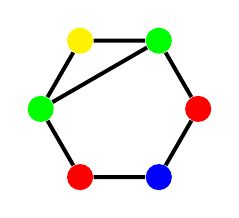
\begin{tikzpicture}[
            scale = 1,
            every node/.style={transform shape, text depth=0pt, circle},
            line/.style={line width = .05cm},
            ]
        
        \node[fill=red] (1) at (0: 1cm) {};
        \node[fill=green] (2) at (60: 1cm) {};
        \node[fill=yellow] (3) at (120: 1cm) {};
        \node[fill=green] (4) at (180: 1cm) {};
        \node[fill=red] (5) at (240: 1cm) {};
        \node[fill=blue] (6) at (300: 1cm) {};
        
        \draw[line] (1) -- (2) -- (3) -- (4) -- (5) -- (6) -- (1);
        \draw[line] (4) -- (2);
    \end{tikzpicture}
    
\end{document}